\begin{frame}{Annexes}
    {Context}

    \begin{block}{Multi-Agent Systems (MAS) paradigm for complex \& distributed problems}
        \begin{itemize}
            \item \textbf{task decomposition}: missions delegated to agents achieved through cooperation~\parencite{Raileanu2023};
            \item \textbf{benefits}: handle conflicting goals, parallel computation, system robustness, scalability\dots
        \end{itemize}
    \end{block}

    \begin{block}{\textbf{Organization}: key for MAS designing}
        \begin{itemize}
            \item \textbf{coordination}: how to collaboratively achieve a common goal~\parencite{Hubner2007};
            \item \textbf{dynamic \& uncertain environments}: flexible runtime behavior to adapt~\parencite{Kathleen2020};
        \end{itemize}
    \end{block}

    \begin{block}{Methods and practice for MAS design}
        \begin{itemize}
            \item \textbf{approach + organizational model}: methods rely on designers' experience to hand-craft agents' \textbf{policies} so resulting MAS achieve goals;
                  %   \begin{itemize}
                  %       \item Examples: \emph{GAIA}~\parencite{Wooldridge2000,Cernuzzi2014}, \emph{ADELFE}~\parencite{Mefteh2015}, or \emph{DIAMOND}~\parencite{Jamont2015}, \emph{KB-ORG}~\parencite{Sims2008}
                  %   \end{itemize}
            \item \textbf{simulation to reality}: 1) safe \& efficient MAS design in high fidelity simulated environment; \quad 2) transfer to real environment to perform adequately~\parencite{Schon2021}.
        \end{itemize}
        \quad $\Longrightarrow$ \textbf{Iterative process proceeding by trial and error}

    \end{block}

\end{frame}

\begin{frame}{Annexes}{CAGE Challenge 3}
    \begin{figure}
        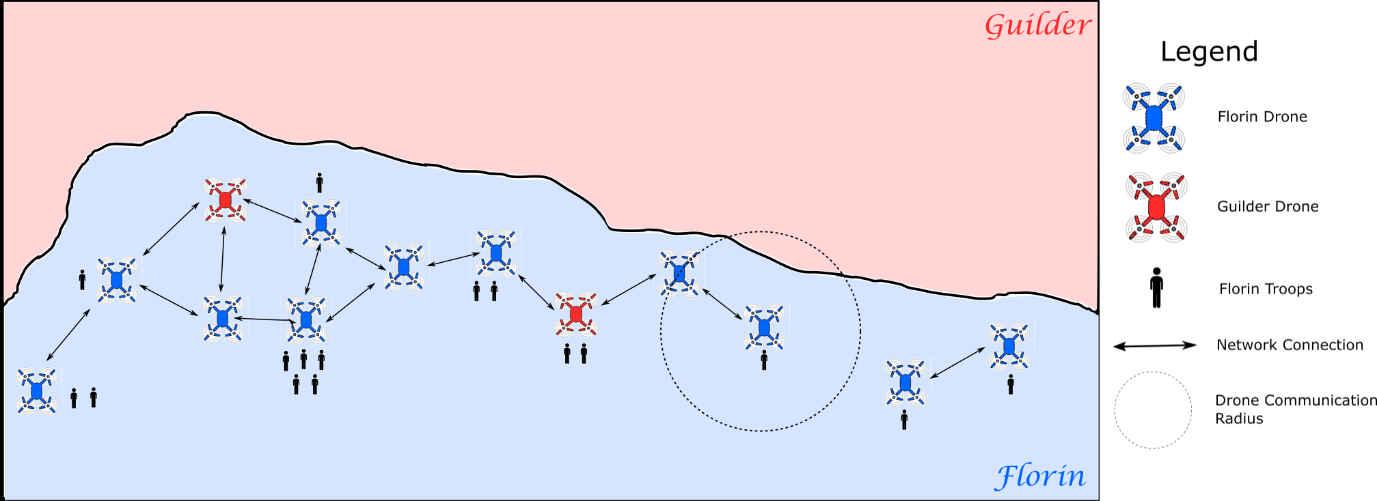
\includegraphics[width=0.9\linewidth]{figures/cage_challenge_3.png}
        \caption*{Florin forces patrolling the Guilder border with troops that communicate via an ad-hoc network provided by aerial drones. Here, Guilder has successfully corrupted two drones within this network and can thus intercept, or alter, some of the messages being communicated.}
    \end{figure}
\end{frame}

\begin{frame}{Annexes}{Prédateur-proie}
    \begin{figure}
        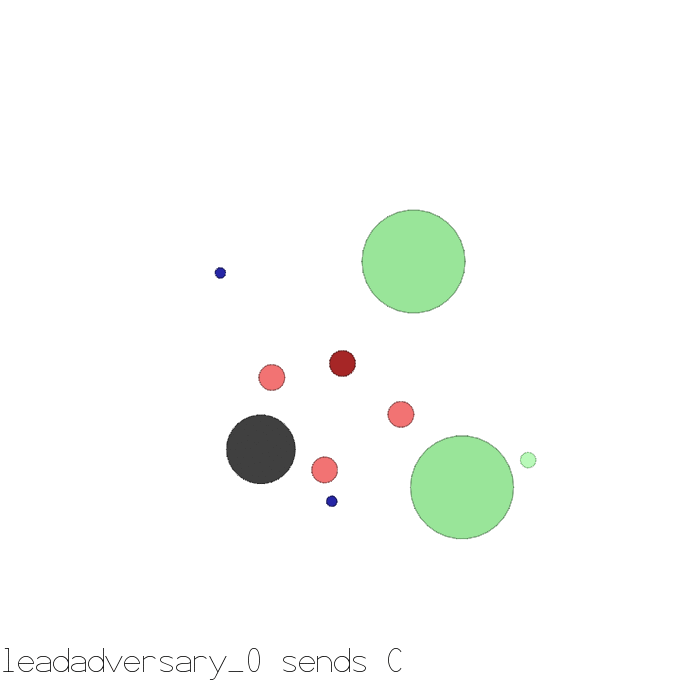
\includegraphics[width=0.5\linewidth]{figures/mpe_simple_world_comm.png}
    \end{figure}
\end{frame}

\begin{frame}{Annexes}{Knight, archers, zombies}
    \begin{figure}
        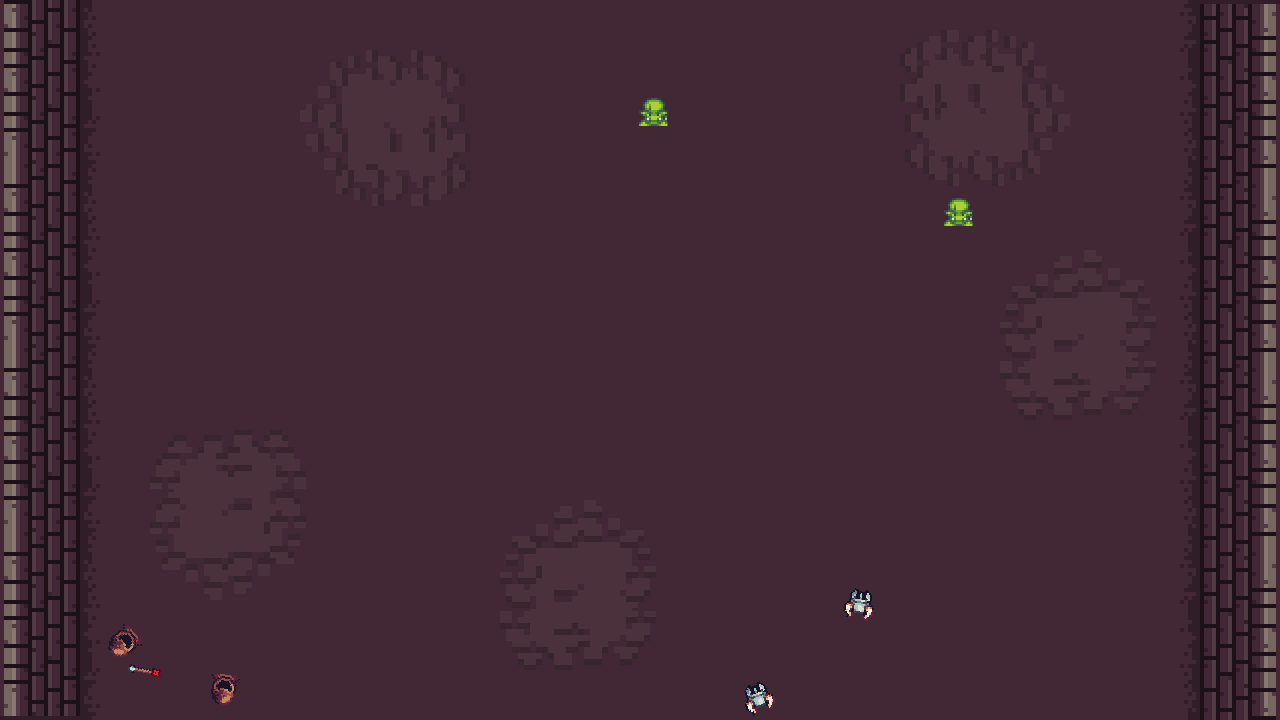
\includegraphics[width=0.8\linewidth]{figures/butterfly_knights_archers_zombies.png}
    \end{figure}
\end{frame}

\begin{frame}{Annexes}
    {MAS basics}

    \begin{block}{Keywords}
        \begin{itemize}
            \item \textbf{Agent}: entity immersed in an environment perceiving observation and making decision autonomously to achieve some goals;
            \item \textbf{MAS}: a set of agents collaborating with self/re-organizing mechanisms to achieve their goal;
            \item \textbf{Organization}: the agents' interactions even though it may be implicit;
            \item \textbf{Organizational Model (OM)}: medium to formally describe an explicit/implicit organization;
            \item \textbf{Organizational Specifications (OS)}: components of an OM to characterize an organization
        \end{itemize}
    \end{block}

    \begin{block}{Organizational model: $\mathcal{M}OISE^+$}
        \begin{itemize}
            \item more complex than \emph{Agent Group Roles} (integration of standards);
            \item takes into account the social aspects between agents explicitly;
            \item possible to link agents' policies to organizational specifications.
        \end{itemize}
    \end{block}

\end{frame}

\begin{frame}{Annexes}
    {MARL basics}

    \begin{block}{Keywords}
        \begin{itemize}
            \item \textbf{Policy}: the \textquote{logic} to choose next action according to observation for an agent;
            \item \textbf{History/trajectory}: the tuple of (observation, action) couples over an episode;
            \item \textbf{Joint-policy / Joint-history}: all of the agents' policies / histories as tuples;
            \item \textbf{Reinforcement learning}: an agent updates its policy to maximize a cumulative reward;
            \item \textbf{Multi-Agent Reinforcement Learning (MARL)}: extends to multiple agents that learn while considering the actions of other agents;
        \end{itemize}
    \end{block}

\end{frame}

\begin{frame}{Annexes}{AOMEA approach: Overview}

    \begin{columns}

        \begin{column}{0.6\textwidth}

            \textbf{Phase 1: Modeling}

            \begin{itemize}
                \item Manually develop a simulated environment ($1.1$) where agents must cooperate to achieve goal ($1.2$);
                \item Can define expected roles behavior as histories;
                \item May constraint agents to roles ($1.3$).
            \end{itemize}

        \end{column}

        \begin{column}{0.4\textwidth}
            \centering
            \adjustbox{trim={0.\width} {0.82\height} {0.\width} {0.\height}, clip}{%
                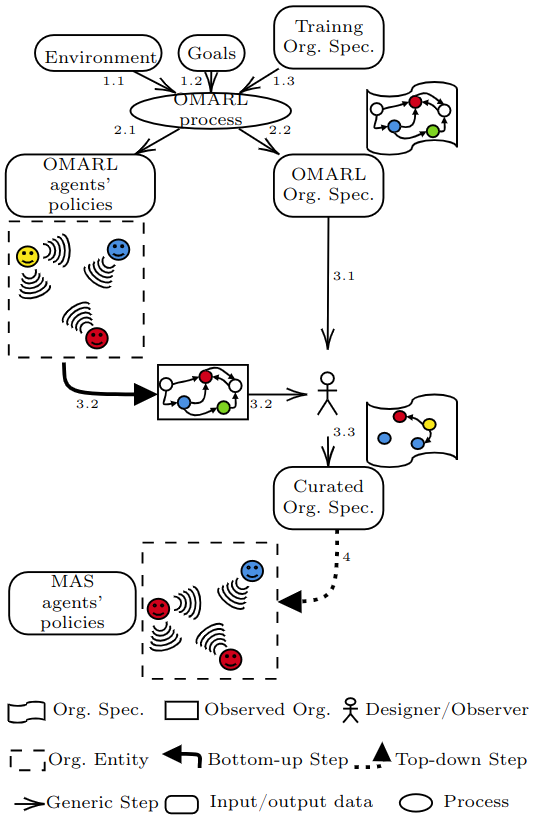
\includegraphics[width=1.2\linewidth]{figures/AOMEA_illustrative_view}
            }
        \end{column}

    \end{columns}

\end{frame}


\begin{frame}{Annexes}{AOMEA approach: Overview}

    \begin{columns}

        \begin{column}{0.6\textwidth}

            \textbf{Phase 2: Solving}

            \begin{itemize}
                \item Organization-oriented MARL (OMARL) algorithm: MARL process augmented with Organizational model;
                \item Solve satisfying constrained roles' histories ($2.1$);
                \item Gets associated OS ($2.2$)
            \end{itemize}

        \end{column}

        \begin{column}{0.4\textwidth}
            \centering
            \adjustbox{trim={0.\width} {0.56\height} {0.\width} {0.\height}, clip}{%
                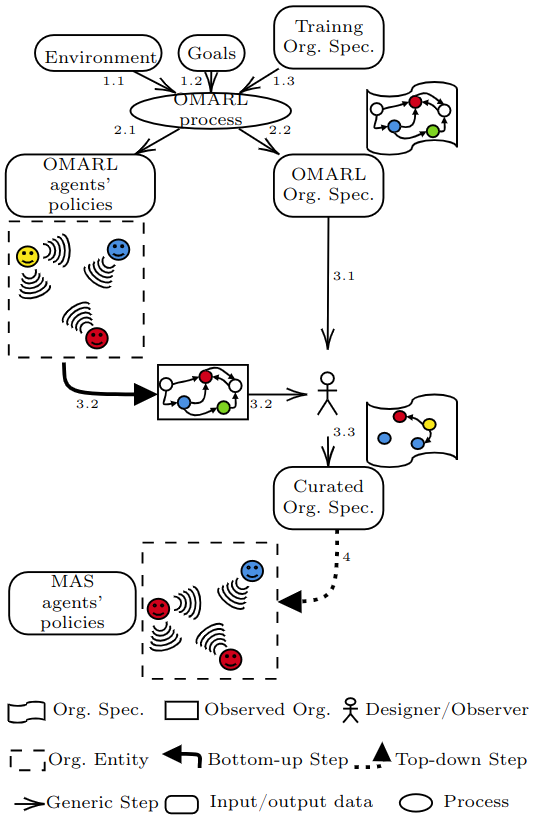
\includegraphics[width=1.2\linewidth]{figures/AOMEA_illustrative_view}
            }
        \end{column}

    \end{columns}


\end{frame}

\begin{frame}{Annexes}{AOMEA approach: Overview}

    \begin{columns}

        \begin{column}{0.6\textwidth}

            \textbf{Phase 3: Analyzing}

            \begin{itemize}
                \item Designers observe the trained agents' policies ($3.2$);
                \item Designers observe the computed OS ($3.1$): understand how they reach the goal;
                \item Designers get some design indications for a MAS to achieve the goal: curated OS ($3.3$).
            \end{itemize}


        \end{column}

        \begin{column}{0.4\textwidth}
            \centering
            \adjustbox{trim={0.\width} {0.35\height} {0.\width} {0.188\height}, clip}{%
                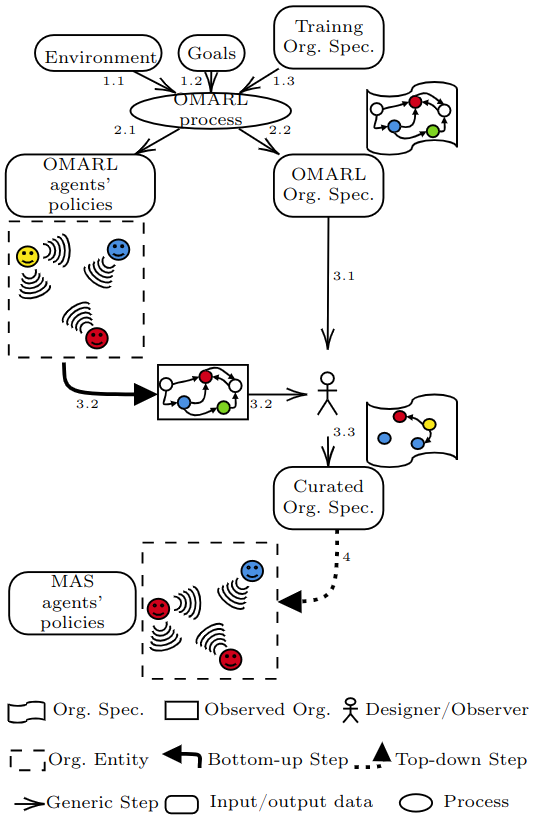
\includegraphics[width=1.2\linewidth]{figures/AOMEA_illustrative_view}
            }
        \end{column}

    \end{columns}

\end{frame}

\begin{frame}{Annexes}{AOMEA approach: Overview}

    \begin{columns}

        \begin{column}{0.6\textwidth}

            \textbf{Phase 4: Developing}

            \begin{itemize}
                \item Designers observe the curated OS for implementing a MAS;
                \item Regular MAS development hence addressing safety issues;
                \item Implemented MAS assessed in simulations.
            \end{itemize}

        \end{column}

        \begin{column}{0.4\textwidth}
            \centering
            \adjustbox{trim={0.\width} {0.15\height} {0.\width} {0.57\height}, clip}{%
                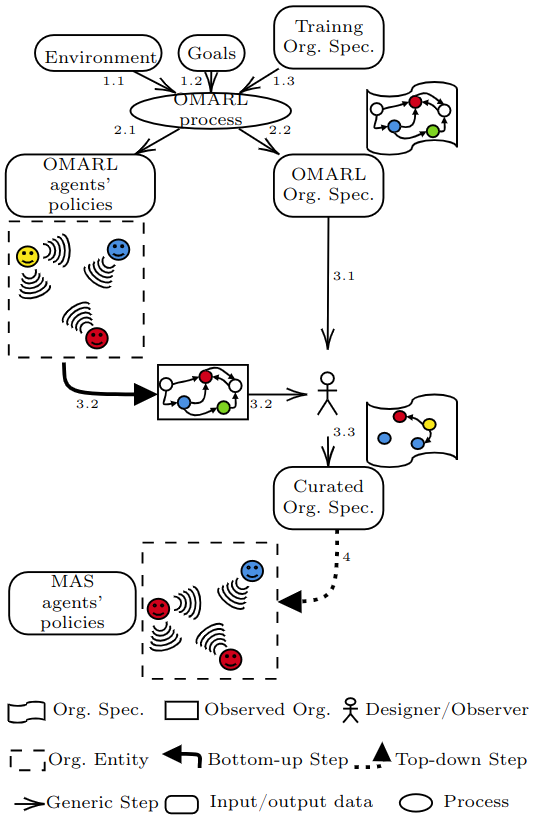
\includegraphics[width=1.2\linewidth]{figures/AOMEA_illustrative_view}
            }
        \end{column}

    \end{columns}

\end{frame}



\begin{frame}{Annexes}{AOMEA approach: Theoretical core}

    \begin{block}{Organization-oriented MARL (OMARL)}
        An MARL process augmented with an OM for:
        \begin{itemize}
            \item \textbf{Constraining Policies Space}: gets the joint-policies satisfying the given design specifications;
            \item \textbf{Inferring Organizational Specifications}: gets the specifications from the agents' policies.
        \end{itemize}

    \end{block}

    \begin{block}{\emph{Partial Relations with Agent History and Organization Model} algorithm (PRAHOM)}
        Implementing an OMARL process\dots
        \begin{enumerate}
            \item \textbf{Constraining Policies Space}
                  \begin{itemize}
                      \item Cannot use policies directly $\rightarrow$ \textbf{histories} characterizing \textbf{policies};
                      \item Relations between \textbf{OS} to expected \textbf{histories};
                      \item Agents constrained to OS $\rightarrow$ at each step: available actions updated regarding \textbf{OS} histories.
                  \end{itemize}

            \item \textbf{Inferring Organizational Specifications}
                  \begin{itemize}
                      \item Analyze histories $\rightarrow$ characterize collective behaviors as OS;
                      \item Using known relations between OS and histories;
                      \item Using general OS definition regarding histories.
                  \end{itemize}
        \end{enumerate}
    \end{block}
\end{frame}

\begin{frame}{Annexes}{AOMEA approach: Theoretical core}

    \textbf{Constraining Policies Space} during training

    \begin{columns}

        \begin{column}{0.3\textwidth}

            \begin{itemize}
                \item At each step, available actions set is changed to match policy constraints defined by users;
                \item Constraints integrated through: external correction, learning, internal policy change.
            \end{itemize}

        \end{column}

        \begin{column}{0.8\textwidth}
            \begin{figure}
                \centering
                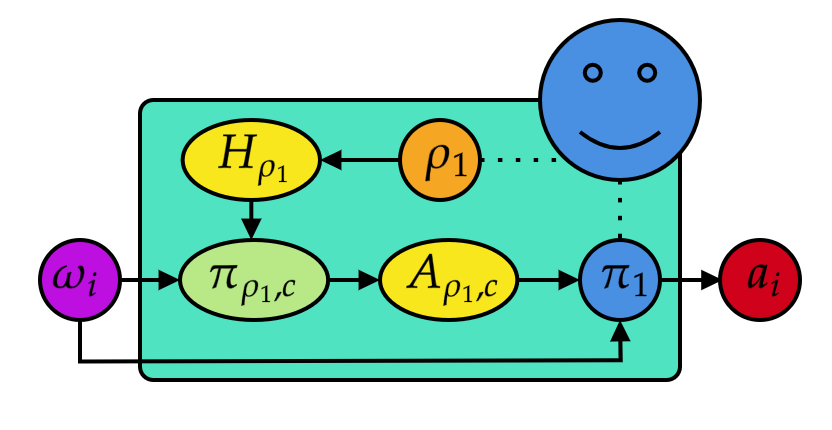
\includegraphics[width=0.7\linewidth]{figures/prahom_training_constrain.png}
                \caption*{A summary view of the PRAHOM constraining}
                \label{fig:prahom_process}
            \end{figure}
        \end{column}

    \end{columns}

\end{frame}


\begin{frame}{Annexes}{AOMEA approach: Theoretical core}

    \textbf{Inferring Organizational Specifications}

    \begin{columns}

        \begin{column}{0.3\textwidth}

            \begin{itemize}
                \item \textbf{Knowledge-based Organizational Specifications Identification (KOSIA)}
                \item \textbf{General Organizational Specifications Infererence (GOSIA)}
            \end{itemize}

        \end{column}

        \begin{column}{0.8\textwidth}
            \begin{figure}
                \centering
                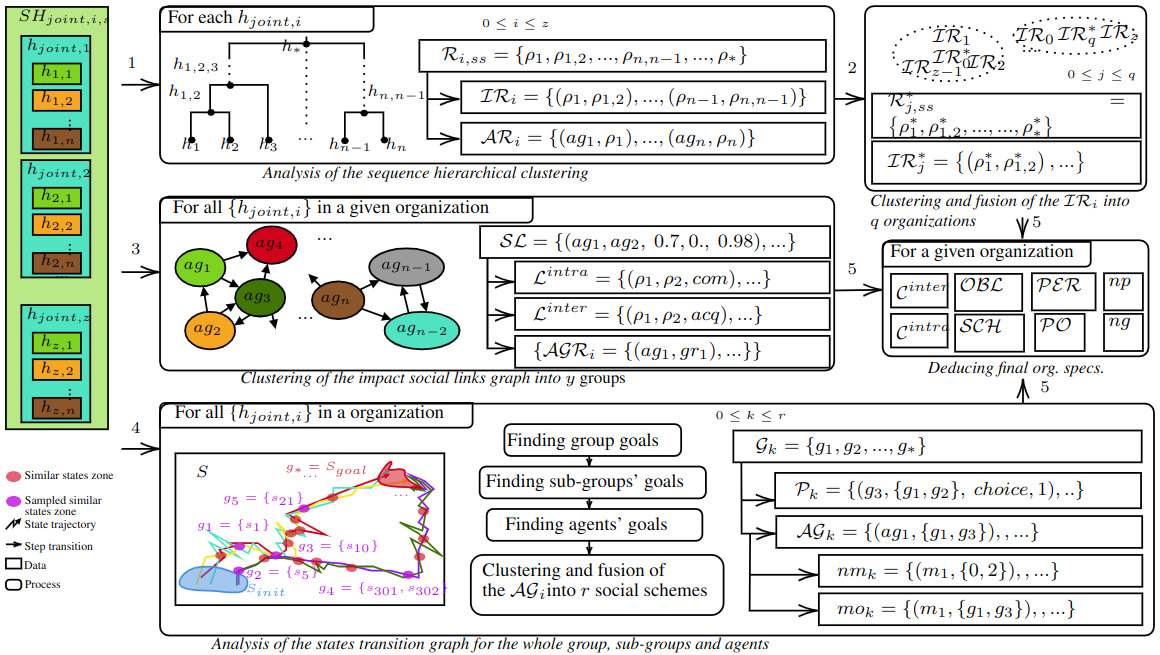
\includegraphics[width=0.95\linewidth]{figures/GOSIA_view.png}
                \caption*{A summary view of the GOSIA process}
                \label{fig:gosia_process}
            \end{figure}
        \end{column}

    \end{columns}

\end{frame}


\begin{frame}[allowframebreaks]{Annexes} {Contexte}

    \begin{block}{Paradigme des Systèmes Multi-Agents (SMA) pour des problèmes complexes et distribués}
        \begin{itemize}
            \item \textbf{décomposition des tâches} : missions déléguées aux agents réalisées par coopération~\parencite{Raileanu2023} ;
            \item \textbf{avantages} : gérer des objectifs contradictoires, calcul parallèle, robustesse du système, évolutivité\dots
        \end{itemize}
    \end{block}
    
    \begin{block}{\textbf{Organisation} : clé pour la conception des SMA}
        \begin{itemize}
            \item \textbf{coordination} : comment atteindre un objectif commun de manière collaborative~\parencite{Hubner2007} ;
            \item \textbf{environnements dynamiques et incertains} : comportement flexible à l'exécution pour s'adapter~\parencite{Kathleen2020} ;
        \end{itemize}
    \end{block}
    
    \begin{block}{Méthodes et pratiques pour la conception des SMA}
        \begin{itemize}
            \item \textbf{approche + modèle organisationnel} : les méthodes s'appuient sur l'expérience des concepteurs pour concevoir manuellement les \textbf{politiques} des agents afin que le SMA atteigne ses objectifs ;
                  %   \begin{itemize}
                  %       \item Exemples : \emph{GAIA}~\parencite{Wooldridge2000,Cernuzzi2014}, \emph{ADELFE}~\parencite{Mefteh2015}, ou \emph{DIAMOND}~\parencite{Jamont2015}, \emph{KB-ORG}~\parencite{Sims2008}
                  %   \end{itemize}
            \item \textbf{simulation vers la réalité} : 1) conception sûre et efficace des SMA dans un environnement simulé à haute fidélité ; \quad 2) transfert à un environnement réel pour des performances adéquates~\parencite{Schon2021}.
        \end{itemize}
        \quad $\Longrightarrow$ \textbf{Processus itératif par essais et erreurs}
    \end{block}

\end{frame}

\begin{frame}[allowframebreaks]{Annexes} {Fondamentaux des SMA}

    \begin{block}{Mots-clés}
        \begin{itemize}
            \item \textbf{Agent} : entité immergée dans un environnement, percevant des observations et prenant des décisions de manière autonome pour atteindre des objectifs ;
            \item \textbf{SMA} : ensemble d'agents collaborant avec des mécanismes d'auto/réorganisation pour atteindre leurs objectifs ;
            \item \textbf{Organisation} : interactions des agents même si elles peuvent être implicites ;
            \item \textbf{Modèle organisationnel (OM)} : moyen de décrire formellement une organisation explicite/implicite ;
            \item \textbf{Spécifications organisationnelles (OS)} : composants d'un OM pour caractériser une organisation.
        \end{itemize}
    \end{block}
    
    \begin{block}{Modèle organisationnel : $\mathcal{M}OISE^+$}
        \begin{itemize}
            \item plus complexe que \emph{Agent Group Roles} (intégration des normes) ;
            \item prend explicitement en compte les aspects sociaux entre les agents ;
            \item permet de lier les politiques des agents aux spécifications organisationnelles.
        \end{itemize}
    \end{block}

\end{frame}

\begin{frame}[allowframebreaks]{Annexes} {Fondamentaux du MARL}

    \begin{block}{Mots-clés}
        \begin{itemize}
            \item \textbf{Politique} : la \textquote{logique} pour choisir la prochaine action en fonction de l'observation pour un agent ;
            \item \textbf{Historique/trajectoire} : le couple (observation, action) sur un épisode ;
            \item \textbf{Politique/historique conjoints} : l'ensemble des politiques/historiques de tous les agents sous forme de tuples ;
            \item \textbf{Apprentissage par renforcement} : un agent met à jour sa politique pour maximiser une récompense cumulative ;
            \item \textbf{Apprentissage par renforcement multi-agent (MARL)} : extension à plusieurs agents qui apprennent en prenant en compte les actions des autres agents ;
        \end{itemize}
    \end{block}
    
\end{frame}

\begin{frame}[allowframebreaks]{Annexes}{Approche AOMEA : Fondement théorique}
    \begin{block}{MARL orienté organisation (OMARL)}
        Un processus de MARL augmenté avec un OM pour :
        \begin{itemize}
            \item \textbf{Contraindre l'espace des politiques} : obtenir les politiques conjointes satisfaisant les spécifications de conception données ;
            \item \textbf{Inférer des spécifications organisationnelles} : obtenir des spécifications à partir des politiques des agents.
        \end{itemize}
    \end{block}
    
    \begin{block}{Algorithme \emph{Partial Relations with Agent History and Organization Model} (PRAHOM)}
        Implémentation d'un processus OMARL\dots
        \begin{enumerate}
            \item \textbf{Contraindre l'espace des politiques}
                  \begin{itemize}
                      \item Impossible d'utiliser directement les politiques $\rightarrow$ \textbf{historiques} caractérisant les \textbf{politiques} ;
                      \item Relations entre \textbf{OS} et historiques attendus ;
                      \item Les agents contraints aux OS $\rightarrow$ à chaque étape : actions disponibles mises à jour en fonction des historiques \textbf{OS}.
                  \end{itemize}
    
            \item \textbf{Inférer des spécifications organisationnelles}
                  \begin{itemize}
                      \item Analyser les historiques $\rightarrow$ caractériser les comportements collectifs comme OS ;
                      \item Utilisation des relations connues entre OS et historiques ;
                      \item Utilisation de la définition générale des OS par rapport aux historiques.
                  \end{itemize}
        \end{enumerate}
    \end{block}
    
\end{frame}

\begin{frame}{Annexes}{Aperçu de \textit{PRAHOM}}
    \begin{figure}
        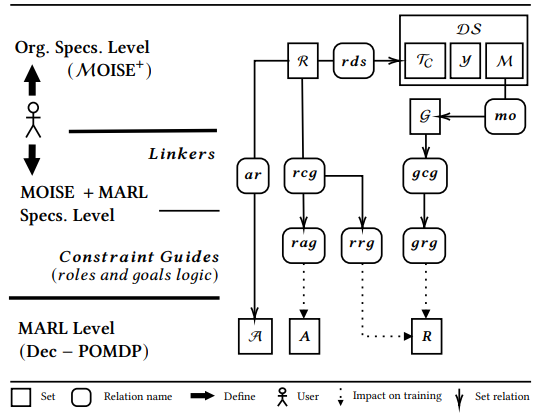
\includegraphics[width=0.6\linewidth]{figures/mm_simple_representation.png}
    \end{figure}
\end{frame}
    
\begin{frame}{Annexes}{Aperçu de PRAHOM}
    \begin{figure}
        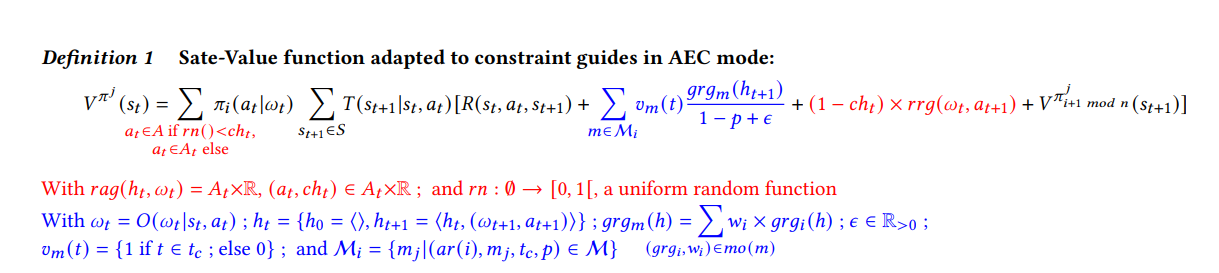
\includegraphics[width=\linewidth]{figures/modified_state_value_function.png}
    \end{figure}
\end{frame}
    
\begin{frame}[allowframebreaks]{Annexes}{Approche AOMEA : Fondement théorique}
    \textbf{Contraindre l'espace des politiques} pendant l'entraînement

    \begin{columns}
    
        \begin{column}{0.3\textwidth}
    
            \begin{itemize}
                \item À chaque étape, l'ensemble des actions disponibles est modifié pour correspondre aux contraintes de politiques définies par les utilisateurs ;
                \item Contraintes intégrées via : correction externe, apprentissage, modification interne des politiques.
            \end{itemize}
    
        \end{column}
    
        \begin{column}{0.8\textwidth}
            \begin{figure}
                \centering
                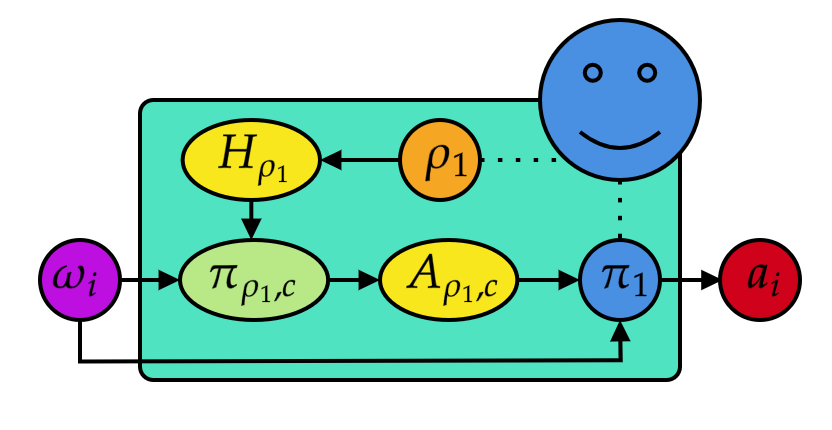
\includegraphics[width=0.7\linewidth]{figures/prahom_training_constrain.png}
                \caption*{Vue résumée de la contrainte PRAHOM}
                \label{fig:prahom_process}
            \end{figure}
        \end{column}
    
    \end{columns}
\end{frame}

\begin{frame}{Annexes}{Constrained Reinforcement Learning (Constrained-RL)}
    
    \begin{itemize}
        \item Apprendre une politique optimisant la récompense tout en respectant des \textbf{contraintes de sécurité} ou de \textbf{performance}.
        
        \item \textbf{Contraintes dures} : doivent toujours être respectées (Shielding).
        \item \textbf{Contraintes douces} : respectées en moyenne ou sous forme de pénalités.
        
        \item \textbf{Méthodes :}
            \begin{itemize}
                \item \textbf{Reward Shaping} : ajout de pénalités pour violation de contraintes.
                \item \textbf{Policy Projection} : ajustement des actions pour rester dans les limites.
                \item \textbf{Dual Variables} : intégration de multiplicateurs de Lagrange pour gérer les contraintes.
            \end{itemize}
            
    \end{itemize}    
\end{frame}

\begin{frame}{Annexes}{Safe Exploration et Shielding en Reinforcement Learning}
    
    \begin{itemize}
        \item \textbf{Safe Exploration} $\rightarrow$ garantir la sécurité lors de la phase d'exploration en limitant les risques de comportements dangereux.
        \item Principalement modifier la fonction de récompense (Langragien) pour integrer contraintes mais aussi\dots
        \item \textbf{Shielding} intervenir en temps réel pour bloquer les actions susceptibles de violer ces contraintes, permettant une exploration sécurisée.
    \end{itemize}
    
    \textbf{Référence :} \\
    \textit{Akifumi Wachi, Wataru Hashimoto, Xun Shen, \& Kazumune Hashimoto (2023). Safe Exploration in Reinforcement Learning: A Generalized Formulation and Algorithms. In Thirty-seventh Conference on Neural Information Processing Systems.}

\end{frame}

\begin{frame}[allowframebreaks]{Annexes}{Approche AOMEA: Fondement théorique}

    \textbf{Inferrer des Spécifications Organisationnelles}

    \begin{columns}

        \begin{column}{0.3\textwidth}

            \begin{itemize}
                \item \textbf{Knowledge-based Organizational Specifications Identification (KOSIA)}
                \item \textbf{General Organizational Specifications Infererence (GOSIA)}
            \end{itemize}

        \end{column}

        \begin{column}{0.8\textwidth}
            \begin{figure}
                \centering
                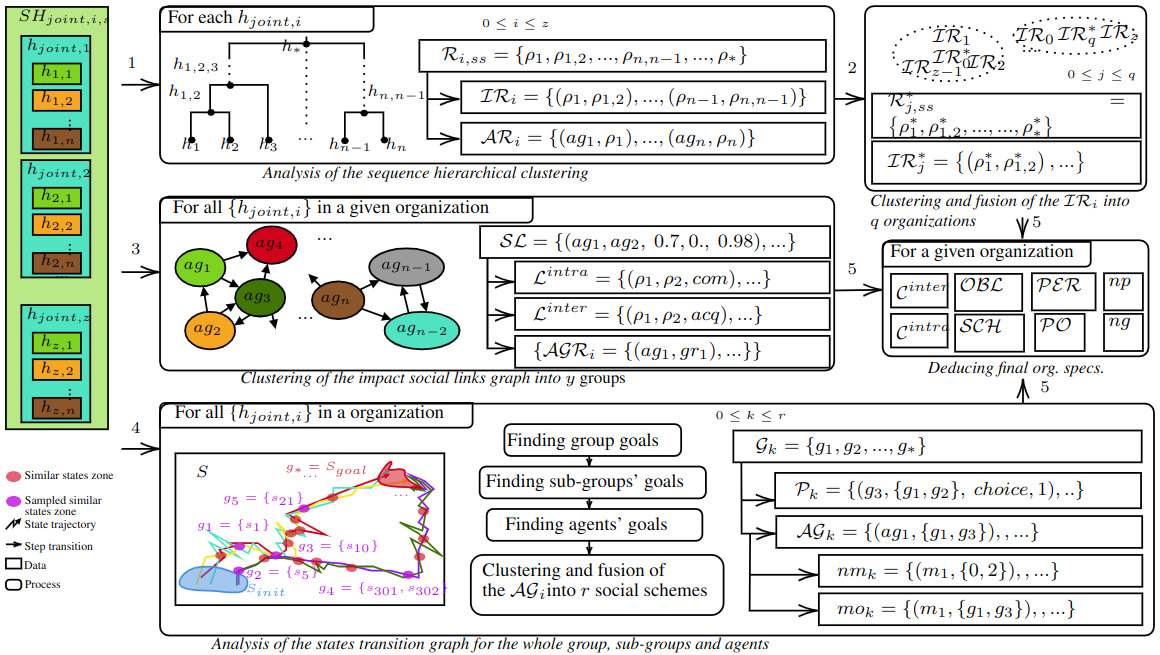
\includegraphics[width=0.95\linewidth]{figures/GOSIA_view.png}
                \caption*{A summary view of the GOSIA process}
                \label{fig:gosia_process}
            \end{figure}
        \end{column}

    \end{columns}

\end{frame}


%%%%%%%%%%%%%%%%

% Slide 2: Exemple d'utilisation
\begin{frame}[fragile]{Annexes}{Exemple d'utilisation d'Optuna}
    \begin{itemize}
        \item \textbf{Optuna} est une bibliothèque open-source pour l'optimisation des hyperparamètres (HPO), utile en apprentissage automatique.
        \item Exemples d'hyper-paramètre : taux d'apprentissage, fonction activation, nb couche, taille couches, seuil de distance pour Hierarchical Clustering\dots
        \item \textbf{Étapes pour utiliser Optuna :}
        \begin{itemize}
            \item \texttt{1.} Définir une fonction d'objectif.
            \item \texttt{2.} Lancer une étude avec Optuna.
            \item \texttt{3.} Utiliser le meilleur résultat pour entraîner le modèle.
        \end{itemize}
    \end{itemize}

    \begin{lstlisting}[language=Python, basicstyle=\small\ttfamily, frame=single, caption=Exemple d'Optuna en Python]
import optuna

def objective(trial):
    x = trial.suggest_float("x", -10, 10)
    return (x - 2) ** 2 # Mock : fonction "etat-valeur"

study = optuna.create_study(direction="minimize")
study.optimize(objective, n_trials=100)

print(study.best_params)  # Affiche les meilleurs parametres
    \end{lstlisting}
\end{frame}


\begin{frame}{Annexes}{Aperçu PettingZoo}
    \begin{itemize}
        \item Bibliothèque Python pour environnements multi-agents.
        \item Simplifier l'entraînement et l'évaluation des agents dans divers environnements.
        \item \textbf{Caractéristiques principales} :
        \begin{itemize}
            \item Supporte plusieurs types d'environnements multi-agents (tour par tour, simultané, etc.).
            \item Intégration facile avec des frameworks de reinforcement learning comme RLlib.
            \item Compatible avec les API de Gym, permettant une utilisation intuitive.
        \end{itemize}
        \item \textbf{Exemples d'environnements inclus} :
        \begin{itemize}
            \item Jeux : \textit{TicTacToe}, \textit{ConnectFour}.
            \item Scénarios de collaboration et de compétition : \textit{Pistonball}, \textit{Prisoner's Dilemma}.
            \item Intégration avec la suite d'environnements Atari pour le multi-agent.
        \end{itemize}
    \end{itemize}
\end{frame}

\begin{frame}[fragile]{Annexes}{Exemple utilisation de PettingZoo}
    \begin{itemize}
        \item Exemple : Création et interaction avec un environnement.
        \item Chargement de l'environnement, réinitialisation et étapes d'interaction pour un agent.
    \end{itemize}
    \vspace{0.3cm}
    \begin{lstlisting}[language=Python, basicstyle=\ttfamily\small]
from pettingzoo.butterfly import pistonball_v6

# Creer et reinitialiser l'environnement
env = pistonball_v6.env()
env.reset()

# Boucle principale d'interaction
for agent in env.agent_iter():
    obs, reward, done, info = env.last()
    action = env.action_space(agent).sample()  # Action aleatoire
    env.step(action)
    if done:
        env.reset()  # Reinitialiser si l'episode est termine
\end{lstlisting}
\end{frame}


\begin{frame}{Annexes}{KB-Org}
    \frametitle{Organization-based multi-agent systems: From modeling to implementation}
    
    \begin{itemize}
        \item Modélisation et mise en œuvre des SMA basés sur organisation ;
        \item Intègre les concepts d'organisation pour structurer les interactions et le comportement des agents ;
        \item Banque d'organisations disponibles prêtes à être utilisé ;
        \item Explicabilité et à la coordination.
    \end{itemize}
    
    \

    Sims, V. (2008). Automated organization design for multi-agent systems. Autonomous Agents and Multi-Agent Systems, 16(2), 151-185.

\end{frame}

\begin{frame}{Annexes}{Présentation de la bibliothèque MARLlib}

    \begin{itemize}
        \item Bibliothèque Python pour MARL
        \item Supporte plusieurs environnements MARL comme PettingZoo, StarCraft II, MPE (Multi-Agent Particle Environment), etc.
        \item Implémente divers algorithmes MARL, incluant MADDPG, MAPPO, etc.
        \item Fournit une interface pour comparaison d’algorithmes, l’entraînement et l’évaluation.
        \item Offre des configurations \textit{fine-tunés} pour de nombreux environnements
    \end{itemize}

\end{frame}

\begin{frame}[allowframebreaks]{Annexes}{Présentation de la bibliothèque MARLlib}

    \begin{itemize}
        \item \textbf{Algorithmes Basés sur les Valeurs}  
        \begin{itemize}
            \item \textbf{Multi-Agent Q-Learning} : Une extension multi-agent fondamentale de Q-learning.  
            \textit{Description} : Simple à implémenter, mais avec des difficultés de scalabilité et de non-stationnarité.
            \item \textbf{MADDPG} : Une adaptation de DDPG pour les environnements multi-agents.  
            \textit{Description} : Gère bien les espaces d'actions continues, mais requiert beaucoup de données et est complexe.
        \end{itemize}
    
        \

        \item \textbf{Algorithmes Basés sur les Politiques}  
        \begin{itemize}
            \item \textbf{REINFORCE} : Une méthode de gradient de politique basique pour l'apprentissage direct de la politique.  
            \textit{Description} : Adaptable aux environnements stochastiques mais souffre de variances élevées des gradients.
            \item \textbf{Multi-Agent PPO (MAPPO)} : Une extension de PPO conçue pour les configurations multi-agents.  
            \textit{Description} : Stabilise les mises à jour, mais nécessite un ajustement minutieux et un coût de calcul élevé.
        \end{itemize}
    
        \item \textbf{Algorithmes Hybrides}  
        \begin{itemize}
            \item \textbf{A3C (Asynchronous Advantage Actor-Critic)} : Combine l'apprentissage des politiques et des valeurs pour un équilibre exploration/exploitation.  
            \textit{Description} : Accélère l'entraînement mais nécessite une synchronisation complexe.
            \item \textbf{MAPPO} : Un hybride intégrant PPO avec un entraînement centralisé.  
            \textit{Description} : Efficace pour les tâches coopératives, mais difficile dans les environnements compétitifs et exigeant en ressources.
        \end{itemize}
    
        \item \textbf{Algorithmes Théoriques et Coopératifs Basés sur le Jeu}  
        \begin{itemize}
            \item \textbf{Independent Q-Learning (IQL)} : Une version indépendante de Q-learning pour chaque agent.  
            \textit{Description} : Simple à implémenter mais avec de sérieux problèmes de non-stationnarité en multi-agent.
            \item \textbf{COMA (Counterfactual Multi-Agent Policy Gradients)} : Utilise des baselines contrefactuelles pour évaluer les contributions des agents.  
            \textit{Description} : Réduit la variance et améliore la coopération, mais demande des calculs lourds.
        \end{itemize}
    
        \item \textbf{Entraînement Centralisé avec Exécution Décentralisée}  
        \begin{itemize}
            \item \textbf{QMIX} : Décompose les valeurs Q pour améliorer la coordination multi-agent.  
            \textit{Description} : Équilibre l'entraînement centralisé et l'action décentralisée, mais moins efficace en environnements très compétitifs.
            \item \textbf{VDN (Value Decomposition Networks)} : Simplifie la coordination multi-agent avec la décomposition des valeurs.  
            \textit{Description} : Efficace mais limité dans la gestion d'interactions complexes.
        \end{itemize}
    \end{itemize}
    

\end{frame}